\documentclass[sigconf,review,anonymous]{acmart}

%% acmart does not load these three.
\usepackage{array}
\usepackage{longtable}
\usepackage{pdflscape}
\graphicspath{{../../}{./}}

%% No author, title or creator metadata keys are set here. acmart drives
%% hyperref itself, and anything set in this preamble reaches the PDF metadata,
%% where it would survive every source-level anonymisation check.

%% A submission carries no DOI, ISBN or price.
\settopmatter{printacmref=false}
\renewcommand\footnotetextcopyrightpermission[1]{}
\acmConference[MSR 2027]{22nd International Conference on Mining Software
Repositories}{April 26--27, 2027}{Dublin, Ireland}

\widowpenalty=10000
\clubpenalty=10000
\setlength{\emergencystretch}{2em}

\title{An arithmetic ceiling on issue--commit linkage, and what it means for corpus selection}

%% The anonymous option suppresses this block; it is kept minimal regardless so
%% there is nothing to leak if the option is ever dropped by accident.
\author{Anonymous Author(s)}

\begin{document}


\begin{abstract}

Empirical studies of architectural change read a project's own records and assume the record traces the work. We measure that assumption on 38 Apache projects.

Two traceability rates diverge. The commit-side rate, the one the literature reports, asks whether a commit cites a ticket. The ticket-side rate asks whether a ticket ever receives a commit, which is what a ticket-anchored design actually needs. Hive cites a ticket in \textbf{97.0\%} of its commits while only \textbf{55.8\%} of its tickets are ever cited by one.

The divergence is arithmetic rather than a matter of discipline. A project supplying \emph{c} commits per ticket cannot realise more than a \emph{c} fraction of its tickets whatever its commit-side rate. Across the twelve eligible projects this ceiling varies \textbf{6.0-fold} while the share of it actually reached varies \textbf{1.19-fold}, so nearly all the spread is supply rather than behaviour. No published linkage rate reports commits per ticket beside it.

Against a bar of 0.80 pre-registered before any project was cloned, \textbf{12 of 38} qualified and none outside a single ecosystem cleared it. We give six mechanisms by which a project silently fails to support an issue-linked study, and none of them is expressible in any published sampling frame.


\end{abstract}


\begin{CCSXML}
<ccs2012>
<concept>
<concept_id>10011007.10011074.10011099</concept_id>
<concept_desc>Software and its engineering~Software verification and
validation</concept_desc>
<concept_significance>500</concept_significance>
</concept>
<concept>
<concept_id>10011007.10011074.10011134</concept_id>
<concept_desc>Software and its engineering~Software evolution</concept_desc>
<concept_significance>300</concept_significance>
</concept>
</ccs2012>
\end{CCSXML}

\ccsdesc[500]{Software and its engineering~Software verification and validation}
\ccsdesc[300]{Software and its engineering~Software evolution}

\keywords{traceability, corpus eligibility, issue linkage, sampling frames,
mining software repositories}

\maketitle


\section{Introduction}
\label{sec:1}

Empirical work on architectural change reads a project's own records --- commit messages, issue trackers, pull requests --- and assumes the record is a reasonably faithful trace of the work. Studies of refactoring motivation, of technical-debt repayment, of architectural erosion and of review effort are all built on that assumption, and it is rarely stated, still more rarely measured. This paper measures it on 38 Apache projects, and finds that the record traces the work far less often than a ticket-anchored design needs, for a reason that is arithmetic rather than cultural.

\textbf{How we arrived at a methods paper.} This study set out to measure signal-to-action latency: what in a project's records precedes a decision to restructure code. Six operationalisations were tried and closed, and Figure~\ref{fig:funnel} records them. The sampling frame turned out to be the finding, and this paper reports that rather than the latency result it went looking for.

\textbf{Contributions.} Stated against what is already published rather than against an assumed gap. We make \textbf{no first-to-measure claim}: Rath \& M\"ader's SEOSS 33 \cite{rath2019seoss} publishes per-project linkage as an explicit table column for 33 projects, and Rath et al. (ICSE'18) \cite{rath2018traceability} publishes both directions for six. An earlier version of this work claimed novelty on that ground; the claim was checked, found false, and withdrawn (\S\kern0.13em \ref{sec:2.1}).

\begin{enumerate}
\item \textbf{A pre-registered numeric eligibility bar, applied before any outcome, with reported attrition and the rejected candidates named.} Prior work selects on trace links informally --- ``a project shall continuously capture trace links'', ``each largely followed the practice of tagging commits with issue IDs'' --- and reports rates afterwards. Neither states a threshold, an attrition count, or which candidates were rejected. Ours is fixed at 0.80, committed before any project was cloned, and never moved.
\item \textbf{A population finding: 12 of 38 pass, and no project outside one ecosystem clears the bar.} The best outside it, James, reaches 74.8\%, against a median of 63.6\% across all 38 and 44.8\% across the 26 rejected. The ecosystem label is a hand classification and we say so: two measured generational variables were tested in its place and neither separates the corpus as well (\S\kern0.13em \ref{sec:4.1}). SEOSS's own table contains the ingredients --- Apache projects at the top, JBoss at the bottom --- but the inference is not drawn there.
\item \textbf{Both reference channels measured together.} Counting GitHub-issue references alongside Jira keys is what shows that the bar selects a \emph{tracker} rather than a discipline: seven of the dropped projects cite GitHub issues in more than half of their commits.
\item \textbf{The arithmetic ceiling that bounds the ticket-side rate}, and the decomposition of that rate into a ceiling set by commits-per-ticket and a residual that measures citation discipline. In this corpus the residual is nearly constant, which is what the divergence actually consists of.
\item \textbf{The ticket-side rate measured across the whole probe rather than only the survivors} --- including the 26 projects that failed the commit-side bar. A strong positive association between the two rates is ruled out; a null is not established, and the live and frozen measurements disagree in sign (\texttt{paper/\allowbreak{}DIRECTION\_\allowbreak{}TENSION.\allowbreak{}md}).
\item \textbf{A six-mode taxonomy of the ways a project silently fails to support an issue-linked study}, three of them disqualifying and three of them producing a plausible wrong number rather than an error.
\end{enumerate}

\textbf{What this paper is not.} It is not a study of refactoring friction; the exploratory Hadoop results live in the replication package and none of them is claimed here. It does not propose the successor design the corpus limits point towards. And it does not argue that the projects it drops are badly run --- a project that moved to GitHub Issues is not failing at anything except a convention this kind of research happens to need.


\section{Related work}
\label{sec:2}

\subsection{Per-project linkage rates are already published}
\label{sec:2.1}

\textbf{This paper makes no first-to-measure claim, and the claim it originally made was withdrawn.} Two prior works publish per-project issue--commit linkage rates, one of them as an explicit table column.

\textbf{Rath \& M\"ader 2019, SEOSS 33} \cite{rath2019seoss} (\emph{Data in Brief} 25:104005) publishes, per project, change-set count and \textbf{``Linked Change Sets [\%]''} for 33 projects --- the same quantity as our commit-side rate. Their spread is 8.11\%--97.13\%; ours is 0.01\%--98.3\% across 38. Four of five overlapping projects agree within \textbf{3.3pp} on corpora seven years apart:

\begin{table*}[htbp]
\centering
\begingroup\footnotesize\setlength{\tabcolsep}{3pt}
\begin{tabular}{>{\raggedright\arraybackslash}p{\dimexpr 0.1911\linewidth-2\tabcolsep\relax}>{\raggedright\arraybackslash}p{\dimexpr 0.3056\linewidth-2\tabcolsep\relax}>{\raggedright\arraybackslash}p{\dimexpr 0.2920\linewidth-2\tabcolsep\relax}>{\raggedright\arraybackslash}p{\dimexpr 0.2113\linewidth-2\tabcolsep\relax}}
\toprule
\textbf{project} & \textbf{SEOSS 2019} & \textbf{this probe 2026} & \textbf{$\Delta$} \\
\midrule
Hadoop & 97.13\% (27,776 commits) & 97.8\% (28,290, 7-key) & +0.7pp \\
Hive & 96.34\% (11,179) & 97.0\% (18,213) & +0.7pp \\
HBase & 90.06\% (14,331) & 92.5\% (21,220) & +2.5pp \\
ZooKeeper & 87.12\% (1,600) & 90.4\% (2,718) & +3.3pp \\
Flink & 41.98\% (12,419) & 66.0\% (38,219) & \textbf{+24.1pp} \\
\bottomrule
\end{tabular}
\endgroup
\end{table*}

That agreement is \textbf{independent cross-corpus validation of the measure} and is treated here as such. Flink's 24.1pp gap is scope rather than error, and unlike in earlier drafts this is now tested rather than asserted: restricting our probe to the \textbf{earliest 12,419 commits} --- the change-set count SEOSS publishes, and the only quantity the two studies share --- gives \textbf{5,214 / 12,419 = 41.9841\%} against their \textbf{41.98\%}, a gap of \textbf{+0.0041pp}. All five overlapping projects agree once scope is matched.

SEOSS's selection criteria matter for our argument: a project must ``continuously capture vertical and horizontal trace links among these artifacts''. So a traceability criterion \textbf{is} used for selection --- but as a qualitative requirement. No cut-off is stated, no rejected candidates are reported, and having selected on trace links the dataset still admits Errai at 8.11\%.

\textbf{Rath et al., ICSE 2018} \cite{rath2018traceability} (\emph{Traceability in the Wild}, arXiv:1804.02433) publishes \textbf{both directions} for six Git+Jira projects, and is the closest precedent to our divergence result. Commit side: ``approximately 48\% of the commits were not linked to any issue'', with a per-project spread from 15\% unlinked in Derby to \textasciitilde{}76\% in Maven. Ticket side: ``approximately 43.3\% of improvements and 42.4\% of bugs have no commits associated with them'' --- Derby works out to 51.8\% ticket-side coverage. Our 12 passing projects run 12.0\%--69.0\% ticket-side, straddling their figure. Their sentence --- ``different practices exist across different projects, leading to huge disparities in the extent to which issue tags are added to commit messages'' --- is our corpus-feasibility finding stated qualitatively in 2018.

Selection there was also informal: the six were chosen because each ``largely followed the practice of tagging commits with issue IDs''. Again no threshold.

\subsection{What is therefore new here}
\label{sec:2.2}

Positioned against the above rather than against an assumed gap:

\begin{enumerate}
\item \textbf{A pre-registered numeric bar applied before any outcome, with reported attrition.} Both prior works select on trace links informally and report the rate afterwards; neither states a threshold, an attrition count, or which candidates were rejected. Ours is fixed in \texttt{predictions/\allowbreak{}PREDICTIONS.\allowbreak{}md} (\texttt{ca076a9}) before any project was cloned, and never moved.
\item \textbf{The population finding.} 12 of 38 pass and no project outside one ecosystem clears the bar. SEOSS's own table contains the ingredients --- Apache at the top, JBoss at the bottom --- but does not draw the inference. The ecosystem label is a hand classification and \S\kern0.13em \ref{sec:4.1} reports the measured variables that failed to replace it.
\item \textbf{Both reference channels measured together.} No prior work counts GitHub-issue references alongside Jira keys, which is what shows the bar selects a \emph{tracker} rather than a discipline.
\item \textbf{The arithmetic ceiling.} The bound TRR $\leq$ CSR $\times$ commits / tickets, the decomposition of the ticket-side rate into that ceiling and a residual, and the finding that in this corpus the residual is nearly constant while the ceiling varies six-fold (\S\kern0.13em \ref{sec:3.1.4}, \S\kern0.13em \ref{sec:4.2}). No prior work reports commits per ticket alongside a linkage rate, which is what makes the two rates look commensurable when they are not.
\item \textbf{The ticket-side rate measured across the whole probe}, including the 26 projects the bar \textbf{rejected} --- Rath 2018 reports it per issue \emph{type}, and only for the six projects it selected. The contribution is the coverage, not the name: \S\kern0.13em \ref{sec:3.1} introduces ``ticket realisation rate'' as a label for the paper's own use and claims no priority for it.
\item \textbf{The six-mode taxonomy}, and that none of it is expressible in any published frame.
\end{enumerate}

\subsection{The standard sampling frame cannot express the criterion}
\label{sec:2.3}

\textbf{Dabic et al. 2021, GHS} \cite{dabic2021sampling} (\emph{Sampling Projects in GitHub for MSR Studies}, MSR'21) is the standard sampling tool and indexes \textbf{735,669 repositories}. A record carries \textbf{35 fields}, queried from the live API rather than read off the paper's Table I, which is an image. Only \textbf{\texttt{totalIssues}} and \textbf{\texttt{openIssues}} touch issues at all, and both are GitHub-issue counts. There is no field for issue-tracker type, external tracker usage, issue--commit linkage, traceability, or commit-message convention. The one adjacent feature, filtering by issue label, is described in the paper as ``still under development''.

The consequence is the actionable one: a researcher sampling with GHS gets stars, commits, contributors and license, then discovers post hoc that 26 of 38 candidates are unusable. That is what happened here.

\subsection{The bug-side linkage literature, and what it already settled}
\label{sec:2.4}

The commit-side/ticket-side asymmetry measured here was studied on the bug side a decade and a half ago. \textbf{Bachmann et al. (FSE'10)} \cite{bachmann2010missing} had a core Apache HTTP Server developer annotate \textbf{493 commits} exhaustively with a purpose-built tool \cite{bird2010linkster}, establishing ground truth rather than inferring it, and found only \textbf{47.6\%} of bug-fix-related commits documented in the tracker; their target is the completeness of the link on one project over one window, ours a per-project rate over a whole tracker, established mechanically. \textbf{Bird et al. (ESEC/FSE'09)} \cite{bird2009fair} is why it matters: missing links are not missing at random, so a dataset built from linked records is a biased sample and models fitted to it inherit the bias, which is the same argument this paper makes for architectural change. Around them, Herzig et al. (ICSE'13) \cite{herzig2013not} show the reports themselves are misclassified, Nguyen et al. (WCRE'10) \cite{nguyen2010case} replicate the bias result, and a line of work beginning with ReLink \cite{wu2011relink} recovers missing links from time proximity, author identity and textual similarity. The two measurements do not condition on the same thing: Bachmann et al. restrict attention to bugs and bug-fix commits, whereas \S\kern0.13em \ref{sec:3.1.1} admits every issue type and conditions on nothing. This paper does not adjudicate whether that makes the quantities distinct, and no claim it makes depends on the answer.

\subsection{Refactoring and self-admitted technical debt}
\label{sec:2.5}

The successor design this corpus limit points towards is a self-admitted technical debt anchor, and its novelty margin rests on three simultaneous choices that the prior work does not combine. That design is not proposed here.


\section{Method}
\label{sec:3}

\subsection{Two traceability rates, and only one of them is published}
\label{sec:3.1}

The literature reports one number and issue-anchored studies depend on another. Both are stated here as definitions so that the divergence in \S\kern0.13em \ref{sec:4} is a comparison between named quantities rather than between two informal readings of the word ``traceability''.

Let \emph{p} be a project with a set of Jira project keys \textbf{$K_p$}, a git repository observed at a pinned commit \textbf{$H_p$}, and a tracker read at a snapshot time \textbf{T}. Write \texttt{cites(c)} for the set of issue keys appearing in commit \emph{c}'s message.

\textbf{Definition 1 --- commit-side rate.} The fraction of commits reachable from $H_p$ whose message cites at least one key with a prefix in $K_p$:

\[\mathrm{CSR}(p) = \frac{\bigl\lvert\{ c : c \longrightarrow H_p, \mathrm{cites}(c) \cap K_p \neq \emptyset \}\bigr\rvert}{\bigl\lvert\{ c : c \longrightarrow H_p \}\bigr\rvert}\]

This is the quantity Rath \& M\"ader publish per project as \emph{``Linked Change Sets [\%]''} (SEOSS 33 \cite{rath2019seoss}) and the quantity Rath et al. (ICSE'18) \cite{rath2018traceability} report as ``approximately 48\% of the commits were not linked to any issue''. It is what the corpus-selection bar in this study is defined on, and it is not novel here.

\textbf{Definition 2 --- ticket realisation rate (TRR).} The fraction of the project's tracked issues that are ever cited by at least one commit:

\[\mathrm{TRR}(p) = \frac{\bigl\lvert\{ k \in \mathrm{Tickets}(p, T) : \exists c \longrightarrow H_p, k \in \mathrm{cites}(c) \}\bigr\rvert}{\lvert \mathrm{Tickets}(p, T)\rvert}\]

TRR is a label of convenience for this paper. It is not a claim to have named the quantity first, and nothing here depends on the name being new. The quantity has been measured before: Rath et al. (ICSE'18) \cite{rath2018traceability} report that ``approximately 43.3\% of improvements and 42.4\% of bugs have no commits associated with them'', as a property of an issue type rather than as a project-level rate, and Bachmann et al. (FSE'10) \cite{bachmann2010missing} measure the completeness of the bug-side link against expert ground truth. What is new here is the use made of the quantity rather than the quantity itself: the divergence between TRR and CSR is not framed anywhere as a constraint on corpus selection.

\textbf{``Realisation'' is a claim about the record, not about the work.} TRR counts a ticket as realised when the repository's own record points back to it. A ticket can be resolved, implemented and shipped without any commit naming it, and such a ticket is counted as unrealised. That is the intended reading: the measure is of what a researcher can \emph{recover}, not of what a project \emph{did}.

\subsubsection{What counts as a ticket}
\label{sec:3.1.1}

Denominator membership is deliberately permissive, because a ticket-anchored study samples from the whole tracker before it knows which tickets are useful:

\begin{itemize}
\item \textbf{All issue types.} Bug, Improvement, New Feature, Task, Test, Wish and Sub-task alike. \textbf{Sub-tasks are included}, because they carry their own key and are cited in commit messages in their own right; excluding them would drop the keys most likely to be cited and inflate the rate.
\item \textbf{All statuses and resolutions.} Nothing is conditioned on \texttt{resolution = Fixed}. This matters for comparability: Vieira et al. (PROMISE'19) \cite{vieira2019reports} select on resolution before measuring, which pre-selects tickets that were worked, so any rate computed that way is not comparable to TRR without adjustment.
\item \textbf{Keys, not names.} Membership is by the issue's key prefix. Measured across the 2,686,282-issue public Jira corpus, 326 project ids carry more than one distinct name while 0 carry more than one key, so a name-based denominator is not stable and a key-based one is (\texttt{paper/\allowbreak{}numbers.\allowbreak{}md} \S\kern0.13em 5).
\item \textbf{Issues that left the project are not in it.} An issue moved out of \emph{p} before T no longer has a \emph{p}-key in the tracker and is not counted; one moved in is counted under its current key. This is a property of the snapshot, not a choice.
\end{itemize}

\subsubsection{What counts as ``ever received a commit''}
\label{sec:3.1.2}

A ticket is realised if \textbf{at least one} commit reachable from $H_p$ carries a token matching \texttt{\textbackslash{}b(?:K1|K2|\ldots{})-\allowbreak{}\textbackslash{}d+\textbackslash{}b} equal to its key, in the commit \textbf{subject or body}. Nothing else is read: not the diff, not the branch name, not a pull request body, not the tracker's own link fields.

The matcher's precision was measured rather than assumed: \textbf{195 of 200 = 97.5\%} (Wilson 95\% CI 94.3--98.9\%) on a seeded 200-commit manual sample across the 12 eligible projects, corpus-weighted 97.7\% (\texttt{paper/\allowbreak{}matcher\_\allowbreak{}validation.\allowbreak{}md}). Two of the five enumerated failure categories could not have fired --- \texttt{version\_\allowbreak{}string} is near-unreachable given a pattern demanding the upper-case key followed by \texttt{-\allowbreak{}} and digits, and \texttt{foreign\_\allowbreak{}key} is unreachable for 11 of the 12, because each project is probed with its own key set and only Ozone is multi-key with both keys its own. \textbf{The single-key $\rightarrow$ multi-key result on Hadoop is therefore not validated by that sample}, Hadoop being the only true monorepo in the study and not among the 12.

One construct limit is recorded rather than corrected: \textbf{a key matched from a branch name counts as a citation.} Merge subjects (\texttt{Merge branch 'master' into KNOX-\allowbreak{}998-\allowbreak{}Package\_\allowbreak{}Restructuring}) and svn trailers (\texttt{.\allowbreak{}.\allowbreak{}.\allowbreak{}/\allowbreak{}branches/\allowbreak{}TEZ-\allowbreak{}1@1471779}) both occur in the sample. The ticket association is correct; the commit need not implement the ticket. The five failure categories were fixed before labelling and do not cover this case, so it was counted genuine and is disclosed here instead of being assigned an invented category.

\subsubsection{How the denominator is bounded in time}
\label{sec:3.1.3}

This is the definitional detail that decides whether TRR is interpretable, and it is the one most easily got wrong.

TRR compares a tracker read at T against a repository read at $H_p$. \textbf{The measure requires T $\leq$ date($H_p$)}, so that every ticket in the denominator has had the whole interval from its creation to date($H_p$) in which to receive a commit. If T runs ahead of the repository, the last tickets filed are structurally incapable of being realised and TRR is biased downward by an amount that depends on the project's filing rate --- an artefact that looks exactly like poor traceability.

Two instantiations are used, and both satisfy the constraint:

\begin{table*}[htbp]
\centering
\begingroup\footnotesize\setlength{\tabcolsep}{3pt}
\begin{tabular}{>{\raggedright\arraybackslash}p{\dimexpr 0.1585\linewidth-2\tabcolsep\relax}>{\raggedright\arraybackslash}p{\dimexpr 0.4223\linewidth-2\tabcolsep\relax}>{\raggedright\arraybackslash}p{\dimexpr 0.2118\linewidth-2\tabcolsep\relax}>{\raggedright\arraybackslash}p{\dimexpr 0.2075\linewidth-2\tabcolsep\relax}}
\toprule
\textbf{} & \textbf{tracker snapshot T} & \textbf{repository $H_p$} & \textbf{coverage} \\
\midrule
\textbf{$\mathrm{TRR}_\mathrm{live}$} & Apache Jira read 2026-\allowbreak{}07-\allowbreak{}25, issue \textbf{keys only} & pinned shas of 2026-\allowbreak{}07-\allowbreak{}25 & the 12 eligible projects \\
\textbf{$\mathrm{TRR}_\mathrm{frozen}$} & the Public Jira Dataset \cite{montgomery2025jira} (Zenodo 15719919), a snapshot predating every pinned sha & the same pinned shas & all 38 probed projects \\
\bottomrule
\end{tabular}
\endgroup
\end{table*}

For \textbf{$\mathrm{TRR}_\mathrm{live}$}, T $\approx$ date($H_p$): the two were read the same day, so the newest tickets are the censored ones and $\mathrm{TRR}_\mathrm{live}$ is a slight underestimate. The restriction to issue keys is enforced mechanically, not by care --- the field list sent to the API is asserted to be \texttt{["key"]}, every returned issue is screened against a forbidden-field set and a hit aborts the run rather than being filtered out, and only the key string survives the parse loop. That is what makes the measurement admissible over a held-out corpus: key existence is not an outcome and nothing in it can be turned into a duration.

For \textbf{$\mathrm{TRR}_\mathrm{frozen}$}, T is years behind $H_p$, which is the safe direction but introduces a different problem: the snapshot's date is not recoverable per project from the parsed artifact. Membership is therefore defined in \textbf{issue-number space} rather than in date space. Jira numbers issues sequentially from 1 within a project, so a tracker holding $N_p$ issues at T holds approximately the first $N_p$ numbers, and the denominator is $N_p$ while the numerator counts only cited keys numbered $\leq$ $N_p$. The two definitions coincide except for issues moved between projects, which perturb the correspondence between count and highest number. \S\kern0.13em \ref{sec:4.3} measures the size of that perturbation rather than assuming it away.

\subsubsection{The arithmetic ceiling, and what is left once it is removed}
\label{sec:3.1.4}

CSR and TRR are not independent quantities, and the constraint between them is exact rather than statistical. It is stated here because \S\kern0.13em \ref{sec:4.2} and \S\kern0.13em \ref{sec:4.3} are organised around it.

A commit either cites no key of \emph{p}, in which case it contributes nothing to the numerator of TRR, or cites at least one --- and however many it cites, it can add \textbf{at most one ticket that no earlier commit had already cited}, in the limiting case where every citing commit introduces a fresh key. So the number of distinct realised tickets is bounded by the number of citing commits:

\[\bigl\lvert\{ k \in \mathrm{Tickets}(p, T) : k \;\mathrm{realised} \}\bigr\rvert \leq \mathrm{CSR}(p) \cdot \lvert C_p\rvert\]

and dividing by |Tickets(p, T)|:

\[\mathrm{TRR}(p) \leq \frac{\mathrm{CSR}(p) \cdot \lvert C_p\rvert}{\lvert \mathrm{Tickets}(p, T)\rvert} \equiv \mathrm{ceiling}(p)\]

The bound is tight --- equality holds when citing commits map one-to-one onto distinct previously-uncited tickets --- and it is reached in practice only if no ticket ever receives two commits.

\textbf{Two consequences, and the second is why this matters.}

First, \textbf{\texttt{commits /\allowbreak{} tickets} is a scale factor the two rates do not share.} A project with 0.16 commits per ticket cannot exceed a 16\% ticket-side rate at \emph{any} commit-side rate, including 100\%. Comparing CSR and TRR without it compares a ratio to a ratio with a different denominator.

Second, it decomposes TRR into a part that is arithmetic and a part that is behaviour:

\[\mathrm{fill}(p) = \frac{\mathrm{TRR}(p)}{\mathrm{ceiling}(p)} \in [0, 1]\]

\texttt{fill} is the share of the attainable maximum actually reached --- how efficiently a project's citing commits spread across distinct tickets rather than piling onto a few. \textbf{\texttt{fill} is the quantity a claim about citation discipline needs}; \texttt{ceiling} is a property of how much code the project writes per ticket it files. Both are reported for every eligible project (Table~\ref{tab:eligibility}). \S\kern0.13em \ref{sec:4.2} shows that in this corpus almost all of the ticket-side variation is ceiling and almost none of it is fill.

\textbf{The subscript propagates, and it matters.} \texttt{ceiling} and \texttt{fill} are both functions of TRR and of the ticket denominator, so each inherits whichever instantiation of \S\kern0.13em \ref{sec:3.1.3} produced it: $\mathrm{ceiling}_\mathrm{live}$ and $\mathrm{fill}_\mathrm{live}$ are computed against the live Jira read of 2026-07-25, $\mathrm{ceiling}_\mathrm{frozen}$ and $\mathrm{fill}_\mathrm{frozen}$ against the frozen snapshot. The two are not interchangeable and they do not always agree about whether the bound binds at all --- three projects have $\mathrm{ceiling}_\mathrm{frozen}$ at or above 100\% while every $\mathrm{ceiling}_\mathrm{live}$ is below it (\S\kern0.13em \ref{sec:4.2}, the artifact's 38-project table). \textbf{Throughout this paper an unsubscripted \texttt{TRR}, \texttt{ceiling} or \texttt{fill} means the quantity in general rather than a measured value; every measured value carries its subscript}, in the prose, in the abstract and in the table captions. Where a project appears with two numbers for what looks like one quantity, the subscripts are the difference.

\subsection{Corpus construction}
\label{sec:3.2}

\textbf{38 Apache candidates}, each Maven-built, Jira-tracked and multi-module. Each was cloned \texttt{-\allowbreak{}-\allowbreak{}filter=blob:none -\allowbreak{}-\allowbreak{}no-\allowbreak{}checkout} --- the probe needs \texttt{git log} and nothing else, so a working tree is pure cost --- and probed with \texttt{scripts/\allowbreak{}traceability\_\allowbreak{}probe.\allowbreak{}py}. Per-project HEAD shas are pinned in \texttt{paper/\allowbreak{}traceability\_\allowbreak{}probe.\allowbreak{}json}, so any re-run is exactly diffable against this one.

\textbf{Hadoop itself is not one of the 38.} It is the corpus the exploratory work was done on, and it is used here only as the worked example for multi-key matching. Every rate reported for the eligible corpus is from a project Hadoop is not.

\textbf{Key prefixes were detected empirically from commit messages, not assumed.} This is not a refinement; it decides the answer. A single-key probe reads Hadoop at \textbf{26.2\%}, against \textbf{92.3\%} on a four-key probe and \textbf{97.8\%} on a seven-key probe of the same 28,290 commits (\S\kern0.13em \ref{sec:5}, modes 5 and 6). The three figures are the same measurement under three key sets, not a rate and a correction to it; 97.8\% is the most complete of them, and the paper quotes whichever key set it names. Evergreen reads 71.7\% under a single-key probe for the same reason. Seven of the 38 needed a second key (\texttt{CALCITE,OPTIQ}, \texttt{HDDS,OZONE}, \texttt{KARAF,FELIX}, \texttt{PINOT,THIRDEYE}, \texttt{ROCKETMQ,RIP}, \texttt{TOMEE,OPENEJB}, \texttt{JAMES,MAILBOX}).

\textbf{One of those second keys was never used.} \texttt{OZONE} appears in Ozone's probed key set and is cited by \textbf{zero} commits; every Jira reference in that repository is an \texttt{HDDS} key. It is retained in the probe because the key set was fixed from a prefix scan before the counts were read, and removing it afterwards would be selection on the outcome. It is also one of \textbf{six} probed keys with no project record in the frozen tracker corpus, which is a different fact about the same key: it is neither cited in git nor present in the tracker.

\textbf{Both reference channels are counted.} GitHub-issue references (\texttt{\#NNN}, \texttt{GH-\allowbreak{}NNN}) are counted per repository alongside Jira keys. This is what turns each drop reason from an inference into a measurement: \texttt{github\_\allowbreak{}issue\_\allowbreak{}references\_\allowbreak{}dominate} means the GitHub count exceeds the Jira count in that repository, and nine projects qualify.

\subsection{The bar, and the discipline around it}
\label{sec:3.3}

\textbf{CSR $\geq$ 0.80}, fixed in \texttt{predictions/\allowbreak{}PREDICTIONS.\allowbreak{}md} (\texttt{ca076a9}) \textbf{before any project was cloned, and never moved.} Lowering it to 60\% would have admitted nine more projects and widened the corpus beyond a single ecosystem. It was not lowered.

The same discipline was applied where it hurt more. A separate frozen threshold --- vendor share $\geq$ 0.40 for the module-tier rule --- was held through a held-out replication in which lowering it would have rescued two of five projects (HBase, maximum share 0.33; Phoenix, which flagged nothing). It was not lowered, and the rule then failed 0 of 3 where it could be tested (\texttt{replication/\allowbreak{}REPLICATION.\allowbreak{}md}). Both facts are stated because a pre-registered threshold that is never tested against temptation is not evidence of anything.

\textbf{Held-out discipline is mechanical.} Outcome data was never observed for seven projects --- Ozone, Tez, ZooKeeper, Ranger, Oozie, Knox, Sqoop. The rule is written down (\texttt{PROJECT\_\allowbreak{}STATE.\allowbreak{}md} \S\kern0.13em 3); the ticket-side script requests one Jira field and aborts if it receives another; the matcher-validation script asks git for \texttt{\%H}, \texttt{\%s} and \texttt{\%b} and nothing else, so it \emph{cannot} compute a duration. HBase and Phoenix were dropped from the held-out corpus on 2026-07-30 and quarantined, because their committed artifacts are one subtraction away from per-ticket latency even though no outcome was ever observed for either; their coverage numbers remain usable and are reported.


\section{Results}
\label{sec:4}

\subsection{Corpus eligibility is the binding constraint}
\label{sec:4.1}

\textbf{Twelve of 38 Apache candidates clear the pre-registered 0.80 commit-side bar, and every one of them is Hadoop-ecosystem under the classification set out below} (Table~\ref{tab:eligibility}, Figure~\ref{fig:funnel}). The bar was fixed before any project was cloned and never moved.

No project outside the Hadoop ecosystem clears it. The best of them, James, reaches \textbf{74.8\%}. The spread runs from ShardingSphere at 0.01\% to Ozone at 98.3\%, with a median of \textbf{63.6\%} across all 38 and \textbf{44.8\%} across the 26 the bar rejected.

\textbf{The ecosystem label is a hand classification, and we tested whether a measured variable does the same work. It does not.} ``Hadoop-ecosystem'' is not a field in any dataset; one of the authors assigned it. The natural replacement is project generation --- free metadata, no judgment, and a mechanism, since projects predating the 2019--20 migration of ASF development to GitHub pull requests had longer under the Jira-citation convention. Two generational variables were tried (\texttt{scripts/\allowbreak{}era\_\allowbreak{}separation.\allowbreak{}py}):

\begin{table*}[htbp]
\centering
\begingroup\footnotesize\setlength{\tabcolsep}{3pt}
\begin{tabular}{>{\raggedright\arraybackslash}p{\dimexpr 0.3782\linewidth-2\tabcolsep\relax}>{\raggedright\arraybackslash}p{\dimexpr 0.1891\linewidth-2\tabcolsep\relax}>{\raggedright\arraybackslash}p{\dimexpr 0.4328\linewidth-2\tabcolsep\relax}}
\toprule
\textbf{variable} & \textbf{coverage} & \textbf{separation} \\
\midrule
Hadoop-\allowbreak{}ecosystem label (hand) & 38 of 38 & accuracy \textbf{0.868}, recall 1.000, precision 0.706, Fisher $p = 2.3$ $\times$ 10$^{-\allowbreak{}}$$^{6}$ \\
repository start year (computed from the clones) & 38 of 38 & AUC \textbf{0.611}, $p = 0.279$, best-\allowbreak{}threshold accuracy 0.711 \\
Apache Incubator graduation date & \textbf{24 of 38} & AUC 0.289, $p = 0.098$, best-\allowbreak{}threshold accuracy 0.625 \\
\bottomrule
\end{tabular}
\endgroup
\end{table*}

Neither generational variable separates the corpus as well as the hand label, and the graduation date is \textbf{missing precisely where it would be needed}: four of the twelve passing projects --- Hive, HBase, ZooKeeper and Ozone --- entered the ASF as Hadoop subprojects rather than as incubator podlings and have no graduation date at all. The free metadata is not free for the group that matters.

\textbf{The drop reasons are measured rather than inferred}, because both reference channels are counted per repository. Nine projects are dropped with \texttt{github\_\allowbreak{}issue\_\allowbreak{}references\_\allowbreak{}dominate}, meaning the GitHub-issue count exceeds the Jira-key count in that repository --- ShardingSphere carries 30,746 GitHub-issue references against 5 Jira keys in 49,111 commits. Four fall in \texttt{below\_\allowbreak{}bar\_\allowbreak{}narrowly} ($\geq$70\%) and the remaining thirteen in \texttt{low\_\allowbreak{}commit\_\allowbreak{}message\_\allowbreak{}hygiene}. Across all 26 the commit-side rate runs \textbf{0.0\%--78.1\%} with a median of \textbf{44.8\%}; the per-project rows are in the replication package.

\subsection{The channel that is published is not the channel that is needed --- and the gap is mostly arithmetic}
\label{sec:4.2}

Across the same twelve projects, the \textbf{commit-side rate runs 82.6--98.3\%} while \textbf{$\mathrm{TRR}_\mathrm{live}$ runs 12.0--69.0\%, with none above 69.0\%} (Definition 1 and Definition 2, \S\kern0.13em \ref{sec:3.1}; Table~\ref{tab:eligibility}). The headline case:

\begin{quote}
\textbf{Apache Hive cites a ticket in 97.0\% of its 18,213 commits, and 55.8\% of its 29,635 tickets are ever cited by one --- $\mathrm{TRR}_\mathrm{live}$.} Nearly perfect commit-side hygiene, and still nearly half the tracker is invisible to a ticket-anchored design.

\end{quote}

\textbf{Most of that gap is not a discipline gap. It is the ceiling (\S\kern0.13em \ref{sec:3.1.4}).} Hive has \textbf{0.61 commits per ticket}, so at 97.0\% commit-side its ticket-side rate cannot exceed \textbf{59.6\%} whatever anyone does --- and it reaches \textbf{0.94} of that. The pattern holds across all twelve:

\begin{itemize}
\item \textbf{$\mathrm{ceiling}_\mathrm{live}$ binds for every one of them}, running 13.7\% (Kylin) to 81.6\% (Ranger) --- a $6.0\times$ spread;
\item \textbf{$\mathrm{fill}_\mathrm{live}$ is flat}: median \textbf{0.89}, range \textbf{0.80} (Ranger) to \textbf{0.95} (Drill), a spread of only \textbf{$1.19\times$};
\item so the $5.8\times$ spread in $\mathrm{TRR}_\mathrm{live}$ is \textbf{$6.0\times$ ceiling and $1.19\times$ fill}.
\end{itemize}

\textbf{Every ceiling in this section is $\mathrm{ceiling}_\mathrm{live}$, and the frozen estimator does not agree that the bound binds.} the artifact's 38-project table computes $\mathrm{ceiling}_\mathrm{frozen}$ against the frozen Jira snapshot and puts three of the twelve at or above 100\% --- Ozone \textbf{176.0\%}, Ranger \textbf{130.4\%}, Knox \textbf{100.0\%} --- where a bound above 100\% does not constrain anything. That is not a disagreement about the projects. It is what a 2026 commit window measured against an older tracker produces: the repository holds more citing commits than the snapshot holds tickets, so the arithmetic ceiling exceeds one and stops being a ceiling. The two estimators bound different denominators, and the note accompanying that measurement says so. Neither figure is withdrawn.

Ranked by fill rather than by rate, the ordering changes almost completely: Drill (43.2\%, fill 0.95) sits above Ranger (65.4\%, fill 0.80). \emph{Every project in the corpus is reaching most of what its commit supply permits.}

\textbf{This is a mechanism, and it replaces the reading the divergence invites.} The tempting story --- ``these projects file tickets they never work on'' --- is not what the numbers show. What they show is that \textbf{a tracker accumulates tickets faster than a repository accumulates commits}, and once fewer than one commit exists per ticket the ticket-side rate is capped below the commit-side rate by construction. The two rates were never commensurable, and reporting one as though it licensed the other is the error, not the projects' behaviour.

\textbf{The consequence for design is unchanged and now has a reason.} A study that samples commits and looks up their tickets can work in any of these twelve. A study that samples tickets and looks for the work is bounded by \texttt{commit-\allowbreak{}side $\times$ commits /\allowbreak{} tickets} before it begins, and that quantity is not reported anywhere in the literature --- including by us, until now.

\subsubsection{Kylin: the sharpest number in the corpus, and why it is withdrawn as the example}
\label{sec:4.2.1}

Earlier drafts led with Kylin --- 83.9\% commit-side against 12.0\% ticket-side, ``seven of every eight tickets with no commit at all''. \textbf{That example is withdrawn.} The pinned commit reaches \textbf{968 commits beginning 2022-08-01}, which is \textbf{7.5\% of the 12,937 commits on the repository's refs}, and the repository itself begins 2014-05-13. The \texttt{apache/\allowbreak{}kylin} default branch was re-initialised for Kylin 5; the earlier history is on other branches.

So Kylin's 12.0\% is measured over a \textbf{four-year commit window against a twelve-year, 5,931-issue tracker}, and its 0.16 commits per ticket --- the lowest in the corpus by a factor of two --- is a fact about the branch, not about Kylin's traceability. Its $\mathrm{fill}_\mathrm{live}$ is \textbf{0.87}, squarely at the corpus median: \emph{by the measure that isolates discipline, Kylin is unremarkable.}

the artifact's 38-project table reports the same project at \textbf{$\mathrm{fill}_\mathrm{frozen}$ 0.00}, and the two are not in conflict. Under the frozen snapshot Kylin's $\mathrm{TRR}_\mathrm{frozen}$ is \textbf{0.04\%} --- two cited keys against a tracker of 4,989 --- because \textbf{99.72\% of its cited keys postdate the snapshot}, so the number cap removes almost the whole numerator. Its $\mathrm{ceiling}_\mathrm{frozen}$ is 16.3\%, well under the bound. The frozen estimator is registering the same truncated branch this section is about, from the other side: live, the window is too short for the tracker; frozen, the tracker is too old for the window. Kylin is the worst end-to-end case in the corpus at 11.91pp (the artifact's 38-project table), and it is flagged in both tables for that reason.

Three other projects have a pinned branch that starts after their repository does --- Jena (49.0\% of refs), Karaf (45.4\%) and James (89.4\%, by eight days) --- and none is near Kylin's severity. The clone-depth column is in \texttt{paper/\allowbreak{}revision\_\allowbreak{}metrics.\allowbreak{}json}; the check is \texttt{scripts/\allowbreak{}revision\_\allowbreak{}metrics.\allowbreak{}py}.

\textbf{Kylin is retained in every table}, because the bar was applied to it before any of this was known and removing it now would be selection on the outcome. It is flagged wherever it appears, and no claim in this paper rests on it.

\subsection{The divergence is a property of the population, not of the survivors}
\label{sec:4.3}

Extending the ticket-side measurement to all 38 probed projects, against a frozen tracker snapshot and with an estimator whose end-to-end error is \textbf{1.76pp mean and 11.91pp maximum}, gives \textbf{no detectable association} between the two rates: $\rho$ = \textbf{$-0.010$} over the 33 projects with a usable denominator, 95\% CI \textbf{$[-0.35, +0.34]$}, permutation $p = 0.958$. That rules out the strong positive relationship a selection bar implicitly assumes, but at 80\% power this study detects only $\lvert \rho \rvert$ $\geq$ \textbf{0.47}, so \textbf{a null is not established}. On the twelve projects measured exactly and live the same correlation is \textbf{$+0.518$}, a disagreement in sign we report rather than resolve, and the per-project rows, the estimator's validation and the sensitivity analyses are in the replication package.

\subsection{The measure replicates independently across corpora seven years apart}
\label{sec:4.4}

The commit-side rate is not a novel measure, and its agreement with an independently constructed dataset is the reason to trust the probe. Four of the five projects overlapping SEOSS 33 agree within \textbf{3.3pp} on corpora seven years apart: Hadoop 97.13\% $\rightarrow$ 97.8\%, Hive 96.34\% $\rightarrow$ 97.0\%, HBase 90.06\% $\rightarrow$ 92.5\%, ZooKeeper 87.12\% $\rightarrow$ 90.4\%.

Flink differed by \textbf{24.1pp} on full history (41.98\% $\rightarrow$ 66.0\%), and the scope explanation for it has now been tested. Re-probing the \textbf{earliest 12,419 commits} --- SEOSS's own change-set count --- gives \textbf{5,214 / 12,419 = 41.9841\%} against their \textbf{41.98\%}: a gap of \textbf{+0.0041pp}, where full history gives +24.1pp. \textbf{Five of five overlapping projects agree once scope is matched.} The remaining 25,800 commits run at 77.62\%, and Flink's by-year series shows why: 0.0\% in each of 2010, 2011, 2012 and 2013, 19.4\% in 2014, 66.0\% in 2015, and 70--88\% every year since (\texttt{paper/\allowbreak{}FLINK\_\allowbreak{}TRUNCATION.\allowbreak{}md}).

\textbf{The exactness of that match is not a warning sign.} The quantity is a deterministic count over a fixed, identically bounded commit range --- not an estimate, and with no sampling error. Two correct implementations of the same well-specified count should agree exactly, and a disagreement would indicate a specification difference rather than noise; exact agreement is only suspicious between estimators that \emph{have} sampling error. The two numbers also arrive by independent paths, one transcribed from a published table and one scanned fresh from a clone at a pinned sha. \textbf{It confirms scope alignment and nothing more} --- in particular it does not validate the ticket-side estimator of \S\kern0.13em \ref{sec:4.3}, which is a different measurement with its own error, reported there.

\subsection{The standard sampling frame cannot express the criterion}
\label{sec:4.6}

GHS is the standard sampling tool for MSR studies. Its 2021 publication reports \textbf{735,669 repositories}; a record returned by the live API in 2026 carries \textbf{35 fields}. (The two figures are of different vintages and are kept apart deliberately: the index has certainly grown since 2021, and the 2021 paper describes 25 characteristics rather than 35.) Only \texttt{totalIssues} and \texttt{openIssues} touch issues at all, and both are GitHub-issue counts. There is no field for issue-tracker type, external tracker usage, issue--commit linkage, traceability, or commit-message convention; the one adjacent feature, filtering by issue label, is described in the paper itself as still under development.

A researcher sampling with GHS therefore gets stars, commits, contributors and license, and discovers post hoc that 26 of 38 candidates are unusable. That is what happened here, and \S\kern0.13em \ref{sec:5} is the taxonomy of the ways it happens.




\begin{figure*}[t]

\centering

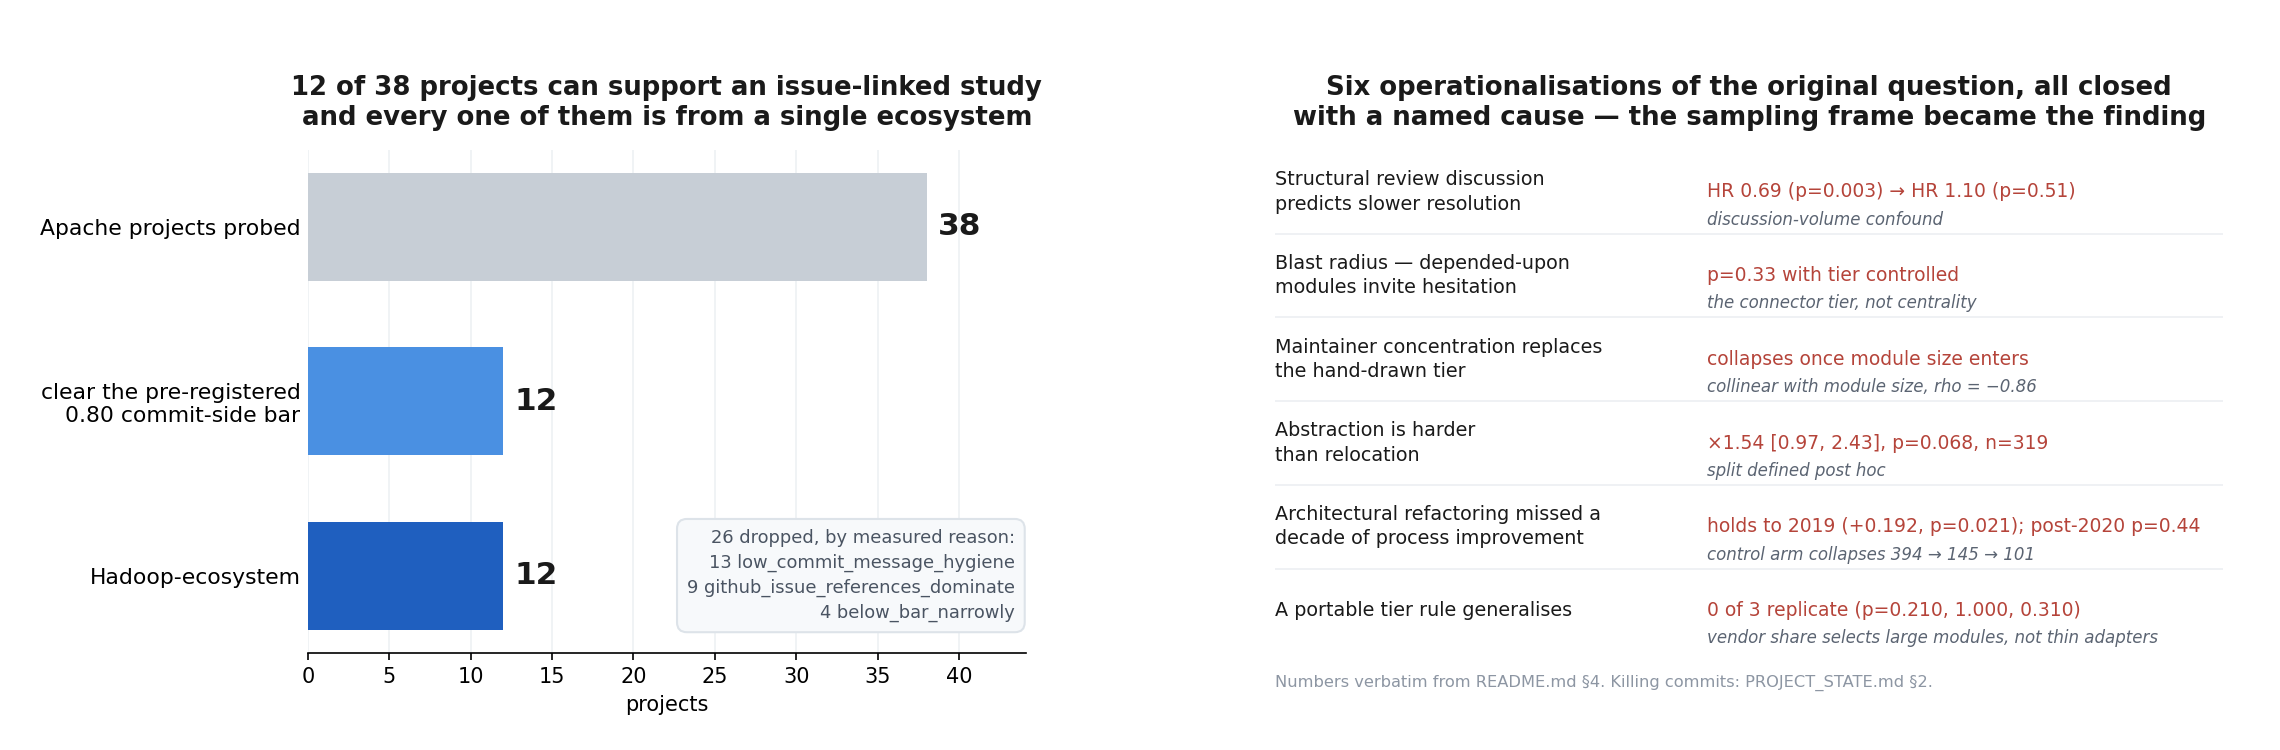
\includegraphics[width=\textwidth]{figures/eligibility_funnel.png}

\caption{Corpus attrition: 38 probed projects to 12 eligible to a single ecosystem, with the six operationalisations that were tested and closed.}\label{fig:funnel}

\end{figure*}



\section{Six ways a project cannot support an issue-linked study}
\label{sec:5}

\textbf{Every mode below was discovered \emph{after} selecting the project, by probing it. None is expressible in any published sampling frame.} GHS indexed 735,669 repositories as published in 2021 and exposes 35 fields per record today, of which only \texttt{totalIssues} and \texttt{openIssues} touch issues, and both are GitHub-issue counts (\S\kern0.13em \ref{sec:2.3}). All six were found the same way: by reading commit messages, project by project.

\begin{table*}[htbp]
\centering
\begingroup\footnotesize\setlength{\tabcolsep}{3pt}
\begin{tabular}{>{\raggedright\arraybackslash}p{\dimexpr 0.0372\linewidth-2\tabcolsep\relax}>{\raggedright\arraybackslash}p{\dimexpr 0.2660\linewidth-2\tabcolsep\relax}>{\raggedright\arraybackslash}p{\dimexpr 0.4461\linewidth-2\tabcolsep\relax}>{\raggedright\arraybackslash}p{\dimexpr 0.2507\linewidth-2\tabcolsep\relax}}
\toprule
\textbf{\#} & \textbf{mode} & \textbf{worked example} & \textbf{evidence} \\
\midrule
1 & \textbf{GitHub Issues displaced Jira} & ShardingSphere: \textbf{5} Jira citations in 49,111 commits, against 30,746 GitHub-\allowbreak{}issue references & \texttt{paper/\allowbreak{}traceability\_\allowbreak{}probe.\allowbreak{}json} \\
2 & \textbf{No source repository exists} & RedHat RHBRMS: 86.00\% estimate coverage on 2,400 issues --- a product/\allowbreak{}documentation tracker with no code & \texttt{estimates\_\allowbreak{}by\_\allowbreak{}org.\allowbreak{}json}; repo resolution failed \\
3 & \textbf{The tracker is downstream of the upstream repo} & kata-\allowbreak{}containers: \textbf{zero} \texttt{KATA-\allowbreak{}} keys in 19,807 commits; the Red Hat Jira tracks a product built from an upstream nobody asks to cite & \texttt{paper/\allowbreak{}intersection.\allowbreak{}json} (excluded, not scored) \\
4 & \textbf{Convention changed mid-\allowbreak{}history} & spring-\allowbreak{}batch: \texttt{BATCH-\allowbreak{}} in \textbf{45.6\%} of 7,035 commits overall, in \textbf{0 of the most recent 1,000} (back to 2021-06), and at exactly \textbf{0\% in every year since 2020} --- a single rate averages two regimes & full scan, \texttt{scripts/\allowbreak{}springbatch\_\allowbreak{}recency.\allowbreak{}py} \\
5 & \textbf{Monorepo needs multi-key matching} & Hadoop: \textbf{26.2\%} single-\allowbreak{}key $\rightarrow$ \textbf{92.3\%} four-key $\rightarrow$ \textbf{97.8\%} seven-\allowbreak{}key, same 28,290 commits & \texttt{scripts/\allowbreak{}citation\_\allowbreak{}rate.\allowbreak{}py} \\
6 & \textbf{The cited key has no project record in the tracker} & Evergreen: commits cite \texttt{DEVPROD} (2,785) but the tracker holds only \texttt{EVG}. DataLab: commits cite \texttt{EPMCDLAB} (3,900) and \texttt{DLAB} (3,547); the tracker holds only \texttt{DATALAB} & \texttt{paper/\allowbreak{}intersection.\allowbreak{}json} \\
\bottomrule
\end{tabular}
\endgroup
\end{table*}

\subsection{The distinction that makes this a taxonomy rather than a list}
\label{sec:5.1}

\textbf{Modes 1, 2 and 3 are disqualifying rather than measurable.} The project is not a weak candidate; it is not a candidate. Scoring kata-containers as ``0\% traceable'' would place it on the same axis as a project that tries and fails, and would put a number where a category belongs.

\textbf{Modes 4, 5 and 6 are silent.} They produce a plausible-looking low number rather than an error. A single-key probe reads Hadoop as 26.2\% and Evergreen as 71.7\%, and \textbf{nothing in either result signals that the key set is wrong.} Four of the 27 projects in \texttt{paper/\allowbreak{}intersection.\allowbreak{}json} needed multi-key matching --- DATALAB (\texttt{DLAB}+\texttt{EPMCDLAB}), TRINIDAD (\texttt{TRINIDAD}+\texttt{ADFFACES}), DAOS (\texttt{DAOS}+\texttt{CART}), EVG (\texttt{EVG}+\texttt{DEVPROD}).

This is the practical consequence, and it is the section's point: \textbf{project eligibility for issue-linked research cannot be established from metadata.} It requires reading commit messages from the project itself, per project, before any outcome is measured.

\subsection{What a sampling frame would need}
\label{sec:5.5}

None of the six is derivable from repository metadata. Expressing them requires, per candidate: the dominant reference channel (Jira keys against GitHub issues, counted rather than assumed), the tracker's project-key set, the key set actually appearing in commit messages, and the rate computed separately over recent history to expose mode 4. All four are cheap. None is in GHS.

\textbf{One qualification, because the unqualified claim overstates the gap.} We say above that the key set cannot be recovered from the tracker, and that stands: a key cited only in git --- \texttt{OPTIQ}, \texttt{EPMCDLAB}, \texttt{DEVPROD} --- is not in the tracker to be enumerated. But a substantial literature \emph{does} recover missing issue--commit links without relying on the commit message, beginning with ReLink \cite{wu2011relink} (Wu et al., ESEC/FSE'11) and continuing since, by learning from time proximity, author identity and textual similarity between report and change (\S\kern0.13em \ref{sec:2.4}). Those methods recover \textbf{links}, not \textbf{key sets}, and they presuppose a project already known to be a candidate --- which is the step this taxonomy is about. Modes 4--6 make a project's \emph{measured rate} wrong; link recovery can raise the true rate afterwards. A sampling frame that exposed the four fields above would tell a researcher which projects are worth pointing a link-recovery tool at, which is a different and prior question.


\section{Threats to validity}
\label{sec:6}

Several of the items below are things this study got wrong and corrected. \textbf{They are stated as the paper's credibility, not as its embarrassments} --- a methods paper about record quality that concealed its own record would be self-refuting.

\subsection{Construct validity}
\label{sec:6.1}

\textbf{The 38-project extension uses a different denominator source, and the validation figure the earlier draft quoted was for a different approximation.} \S\kern0.13em \ref{sec:4.3} measures the ticket realisation rate for all 38 projects against the frozen public Jira corpus rather than a second live fetch, aligning numerator and denominator in issue-number space (\S\kern0.13em \ref{sec:3.1.3}). \textbf{Two approximations are stacked}: number-capping, and substituting a frozen snapshot for the live tracker. The 0.45pp / 2.14pp figure earlier drafts quoted validates only the first. The end-to-end error of the combination the artifact's 38-project table actually uses is \textbf{1.76pp mean / 11.91pp max}, the worst case being Kylin; excluding Kylin it is 0.84pp mean and \textbf{2.93pp max, with 11 of 12 inside 3pp}. \textbf{Quote the end-to-end figure.}

\textbf{And the estimator is applied entirely outside its validated range.} The twelve validation projects span commit-side \textbf{82.6--98.3\%}; the twenty-one that carry the \S\kern0.13em \ref{sec:4.3} association span \textbf{10.5--78.1\%}. The ranges are \textbf{disjoint --- 0 of 21} applied projects fall inside the validated one. The error mechanism is tracker-numbering density rather than commit hygiene, and within the twelve the error does not track the commit-side rate ($\rho = -0.16$, $n = 12$), so there is a reason to expect the extrapolation to hold --- but it is a reason, not a validation, and \textbf{any claim whose margin is smaller than 11.91pp is not safe on this estimator.} The claims that are: the ceiling identity (exact arithmetic, not estimated); the eligibility result (commit-side only); the taxonomy. The claims that are not: any per-project ticket-side comparison in the artifact's 38-project table closer than \textasciitilde{}12pp, and the passing-versus-dropped median gap of 0.6pp, which is far inside the noise and is reported as such.

Four further things can break the estimator, and all four occur in this corpus:

\begin{enumerate}
\item \textbf{Trackers with gaps.} Number-capping assumes a tracker holding N issues holds approximately the first N numbers. Issues moved or deleted break that, and the estimator then undercounts. This is the largest single validation error in the set and the direction is always downward.
\item \textbf{Repositories whose history does not span the snapshot era.} Where a repository has been truncated or re-initialised, almost none of its cited keys fall inside the frozen range and the estimated rate collapses towards zero. That is a \emph{true} statement about what is recoverable from the repository as it now stands, and a badly misleading one if read as a statement about whether the project's tickets were ever worked. Affected projects are flagged in the artifact's 38-project table with the share of cited keys that postdate the snapshot --- \textbf{99.72\% for Kylin (709 of 711), not 100\%}; an earlier draft printed 100\%, which contradicts the non-zero numerator that produces Kylin's 0.04\%.
\textbf{This defect is not confined to the frozen arm, and that is the more serious finding.} Kylin's pinned commit reaches \textbf{968 commits beginning 2022-08-01}, \textbf{7.5\% of the 12,937 on the repository's refs}, against a tracker of 5,931 issues and a repository that begins 2014-05-13. Its \emph{live} 12.0\% is therefore also measured over a four-year window against a twelve-year tracker. Earlier drafts made that 12.0\% the paper's flagship example while dismissing the frozen 0.04\% as an artefact; \textbf{both are the same artefact}, and the example has been moved to Hive (\S\kern0.13em \ref{sec:4.2.1}). Three other projects have a pinned branch starting after their repository --- Jena (49.0\% of refs), Karaf (45.4\%), James (89.4\%, by eight days) --- and none approaches Kylin's severity (\texttt{scripts/\allowbreak{}revision\_\allowbreak{}metrics.\allowbreak{}py}).

\item \textbf{Denominators too small to carry a rate.} Several trackers hold only a handful of issues in the frozen corpus. Projects with fewer than 500 are excluded from the association statistic and shown in the table with the exclusion marked.
\item \textbf{Keys with no tracker record at all.} Some probed keys have no project record in the frozen corpus. These are taxonomy modes 1 and 6, not low rates, and they are \textbf{excluded rather than scored as 0\%} --- scoring them would put a number where a category belongs, which is the error \S\kern0.13em \ref{sec:5.1} exists to prevent.
\end{enumerate}

\textbf{The truncation caveat on Table~\ref{tab:eligibility} is not withdrawn.} The 12.0--69.0\% range from the live measurement remains within-passing variation, computed on the twelve that had already cleared the bar. \S\kern0.13em \ref{sec:4.3} does not extend that measurement; it is a different estimator against a different snapshot, and it is reported alongside rather than merged into it.

\subsection{Single-rater limits, and the one measure that escapes them}
\label{sec:6.5}

\textbf{Inter-rater agreement cannot be computed by one person, so no measure requiring manual coding carries a claim in this paper.} Two instruments are affected and both are reported \textbf{as findings about the instrument}, never as instruments the paper's claims rest on:

\begin{itemize}
\item the codebook's keyword rule for structural review discussion --- \textbf{$\approx$25\% precise} (5 of 20 flagged comments genuinely structural), $\approx$5\% miss (1 of 20 unflagged), on a 40-comment single-rater pass, with no $\kappa$;
\end{itemize}

Its role is to establish that keyword-based detection over-counts roughly fourfold, which is a validity result about a method other studies use.

\textbf{The exception is argued rather than asserted.} The 200-commit matcher check is a mechanical determination against a written rule with categories fixed before labelling, not a coded judgment where the construct lives in the rater's head. It is made \textbf{auditable rather than agreed}: \texttt{paper/\allowbreak{}matcher\_\allowbreak{}sample.\allowbreak{}json} carries all 200 messages and \texttt{paper/\allowbreak{}matcher\_\allowbreak{}labels.\allowbreak{}json} every label, so any reader can re-check the sample without redrawing it.

\textbf{The architectural-episode gold set has no second rater and is therefore not used} to support any claim here.

\textbf{One coincidence in the rater pilot is disclosed because it looks like tuning and we cannot prove it is not.} \texttt{paper/\allowbreak{}LLM\_\allowbreak{}RATER\_\allowbreak{}PILOT.\allowbreak{}md} reports that six comments change label under the opposite ordering of two codebook rules, and \textbf{five of the six fall in the flagged bucket} --- the margin moves 3/12/5 to 3/7/10, a swing of exactly five. The $\kappa$ ceiling is computed on that bucket, so five is the count that drives it, and five moves the attainable ceiling from 0.491 to \textbf{0.840}. \emph{(Corrected 2026-08-05: this paragraph previously credited the 0.840 to the six re-labelled comments. Six is the total across both buckets; the ceiling is indexed by flagged-bucket moves alone. No figure changes.)}

\textbf{Five is also exactly the count that maximises the ceiling over every possible count}: four gives 0.765, six gives 0.837, seven gives 0.833. The six were selected by a stated semantic criterion, they are individually defensible, and the finding is robust at 0.833--0.840 across plus or minus two comments --- but the criterion was applied by the same party that reported the resulting number, and it landed on the global maximum. Stated here rather than left for a reader to find (\texttt{audit/\allowbreak{}JUDGMENTS.\allowbreak{}md} \S\kern0.13em 3).

\subsection{External validity}
\label{sec:6.7}

\textbf{One mined project, one ecosystem.} All 12 eligible projects are Hadoop-ecosystem, and depth beyond Hadoop was not reachable. The corpus bound is therefore a finding and a limit at once: results about Apache/Jira/Java traceability generalise to Apache/Jira/Java.

\textbf{At 12 projects the design is not powered, whatever the corpus size.} Effective n is capped at P/ICC by between-project correlation --- a ceiling of 600 at ICC 0.02 against the 769 the effect needs. The direction of the bias is bad: these twelve share contributors, committers, review norms and in several cases build and CI infrastructure, so this sample's ICC is higher than a random sample's. \textbf{The ICC itself is unmeasured, and was deliberately not estimated from the four available clusters}, because between-cluster variance is not estimable at $n=4$ and the estimate must come from the pooled study as a first stage (\texttt{replication/\allowbreak{}CORPUS\_\allowbreak{}FEASIBILITY.\allowbreak{}md}).


\section{Discussion}
\label{sec:7}

\subsection{For researchers designing an issue-anchored study}
\label{sec:7.1}

\textbf{Project eligibility cannot be established from metadata.} Every one of the six failure modes in \S\kern0.13em \ref{sec:5} was found by reading commit messages from the project itself, after the project had been selected. Three of them are silent: they yield a plausible low number rather than an error, and nothing in the result signals that the key set is wrong. A researcher who samples on stars, contributors and language, then computes a linkage rate, will get a number for every candidate and will not be told which of those numbers mean anything.

\textbf{Measure the side of the rate your design actually samples on, and report commits per ticket beside it.} A commit-side rate answers ``if I start from a commit, can I find its ticket?''. A design that starts from \emph{tickets} needs the ticket realisation rate, and the first does not imply the second --- Hive is 97.0\% one way and 55.8\% the other ($\mathrm{TRR}_\mathrm{live}$). But the more useful advice is the ceiling (\S\kern0.13em \ref{sec:3.1.4}): \textbf{below one commit per ticket the two rates are not commensurable at all}, and every project in our eligible corpus is below it. Report \texttt{commits /\allowbreak{} tickets}; it costs nothing, it bounds the ticket-side rate before any measurement, and no published linkage rate carries it.

\textbf{What our own extension does and does not license.} Across the whole probe we find no detectable association between the two rates ($\rho = -0.010$, $n = 33$, 95\% CI $[-0.35, +0.34]$). That rules out a strong positive relationship --- the assumption a selection bar encodes --- but at 80\% power this study detects only $\lvert \rho \rvert \geq 0.47$, so it does not establish a null. On the twelve projects measured exactly the same correlation is $+0.518$, and we report the disagreement rather than resolving it (\texttt{paper/\allowbreak{}DIRECTION\_\allowbreak{}TENSION.\allowbreak{}md}).

\textbf{Report the bar, the attrition, and the rejected candidates.} The dropped projects are the informative part. That 26 of 38 Apache candidates are unusable, and that the 12 survivors are one ecosystem, is a fact about the population that a paper reporting only its final corpus cannot convey --- and it is a fact each such paper independently rediscovers and does not write down.

\subsection{For dataset and sampling-frame builders}
\label{sec:7.2}

The fields that decide usability are absent from the standard frame. GHS indexed 735,669 repositories as published in 2021 and exposes 35 fields per record today; only \texttt{totalIssues} and \texttt{openIssues} touch issues and both are GitHub-issue counts. There is no tracker type, no external tracker, no issue--commit linkage, no commit-message convention.

Four fields would close most of the gap, and all four are cheap to compute from a shallow clone and a tracker listing:

\begin{enumerate}
\item \textbf{the dominant reference channel} --- Jira-key citations against GitHub-issue references, \emph{counted}, not assumed;
\item \textbf{the tracker's project-key set}, which catches concurrent siblings (mode 5);
\item \textbf{the key set actually appearing in commit messages}, which is the only thing that catches superseded records (mode 6) --- those keys exist in git and nowhere else;
\item \textbf{the rate recomputed over recent history}, which exposes a convention that changed mid-history (mode 4).
\end{enumerate}

\textbf{What the four fields would cost.} All four come from a \texttt{-\allowbreak{}-\allowbreak{}filter=tree:0} bare clone plus one tracker listing. On this corpus those 38 clones came to \textbf{228 MB, a mean of 6.0 MB per project}, against the 4.3 GB the original working-tree sweep took --- a 19x reduction. Fields 1, 3 and 4 need only \texttt{git log} over commit messages --- no trees, no blobs, no working tree. Field 2 is one paginated tracker call for issue keys. For a frame that already crawls repository metadata at the scale of 735,669 repositories, the marginal cost is the clone, and the clone is the cheapest kind there is. We are not claiming it is free at that scale; we are claiming it is the same order as what GHS already does per repository, and that nobody has to guess.

This study spent 38 clones and 4.3 GB to keep 12. That cost is paid again by every group that attempts the same kind of corpus, and none of it is recoverable from published metadata.

\subsection{What follows from the corpus limit, without softening it}
\label{sec:7.4}

A corpus bounded to one ecosystem cannot support the between-ecosystem comparison the design wanted, and there are three ways out, each with a cost: \textbf{lower the bar and model the measurement error}, which buys nine more projects at the price of a biased sample of tickets within each; \textbf{change the outcome so it needs no tickets}, which dissolves the problem and the creation-to-first-commit clock with it; or \textbf{accept ecosystem-bounded scope and say so}. The third is the honest one and is what we do.

\subsection{What this paper does not claim}
\label{sec:7.5}

It does not claim that Jira-citing projects are better engineered, or that the projects on GitHub Issues are less traceable in any sense that matters to their own maintainers. The convention this research needs is not a quality signal; it is a research affordance, and its decline is a cost to researchers rather than to the projects.

It does not propose the successor design that the corpus limits point towards. That is a separate registered report with its own feasibility gates, and its novelty margin against an active architectural-debt time-to-fix literature is recorded in the replication package as \textbf{not assessed}.

And it does not offer a fix. The six modes are diagnosable, not repairable: a project whose tracker is downstream of its repository will not start citing keys because a researcher would like it to.


\section{Acknowledgements and disclosures}
\label{sec:8}

\subsection{Data availability}
\label{sec:8.1}

Every artifact this paper rests on is archived and citable: the 38 pinned repository shas, the frozen tracker caches, the per-project measurements, the full 38-row eligibility table, the three-channel visibility table, every script that produced a number here, and the audit report against which the numbers were re-derived. \textbf{Replication package: ANONYMISED-ARTIFACT-DOI.} Nothing needed to reproduce a figure in this paper lives only in a version-control host.

\subsection{Data and tools}
\label{sec:8.2}

This study is built on artifacts other people made public. The Apache Software Foundation publishes the issue trackers and repositories the whole corpus is drawn from. Lloyd Montgomery, Clara L\"uders and Walid Maalej deposited the Public Jira Dataset (Zenodo 15719919, CC BY 4.0), which supplies every estimate-coverage base rate and every frozen ticket denominator in the artifact's 38-project table. Michael Rath and Patrick M\"ader's SEOSS 33 provides the independent measurement this study's probe is validated against, and the agreement between them at matched scope (Section~\ref{sec:4.4}) is the strongest external check the work has. Nikolaos Tsantalis and the RefactoringMiner contributors built the detector. None of them is responsible for what is done with their work here.

\subsection{Use of AI tools}
\label{sec:8.3}

\textbf{Declared in full, because a paper about the trustworthiness of records should be candid about how its own were produced.}

Large language model assistants (Anthropic's Claude) were used across parts of this work. Their role was:

\begin{itemize}
\item \textbf{writing and running analysis code.} Every script in \texttt{scripts/\allowbreak{}} that produced a number in this paper was drafted with assistance. The scripts are committed, the artifacts they emit are committed, and each is re-runnable --- that is what makes the assistance auditable rather than something the reader must take on trust.
\item \textbf{drafting prose.} The manuscript sections were drafted with assistance from the author's outlines, findings and decisions, and revised by the author.
\item \textbf{literature verification.} Citations were checked against source texts --- authors, venue, year, identifier, and whether the source says what is attributed to it. The record of those checks is in the replication package.
\item \textbf{an adversarial audit of this work's own numbers.} An independent AI-conducted pass re-derived the load-bearing results from primary artifacts with separately written code, exhaustively enumerated the $\kappa$ bounds, verified all 2,491 frozen cache files against their manifest, and reported what it found --- including several errors that were then corrected. Its report is in the replication package under \texttt{audit/\allowbreak{}}, unedited.
\end{itemize}

\textbf{What the tools did not do.} The research questions, the study design, the pre-registered 0.80 bar and its commitment before any project was cloned, the decision to hold that bar and the vendor-share threshold when moving them would have helped, the six retractions, and the judgment of what the results mean are the author's. \textbf{The author takes full responsibility for all content, including any error a tool introduced and the author did not catch.}

\emph{A line-by-line verification checklist for this section, separating what is observable in the repository's record from what is inferred about the sessions that predate it, is at \texttt{paper/\allowbreak{}DISCLOSURE\_\allowbreak{}VERIFICATION.\allowbreak{}md}.}

\textbf{Errors that assistance introduced and review caught} are recorded rather than quietly fixed, because they bound how much the audit trail is worth: a median computed as the upper-middle value at even \emph{n}; a validation figure quoted for a different approximation than the one in use; a provenance checker that could not fail, and a first rebuild of it that reproduced the same defect by another route. Each is in \texttt{paper/\allowbreak{}REVISION\_\allowbreak{}LOG.\allowbreak{}md} with what it changed.

\subsection{A separate matter: the LLM used as a rater}
\label{sec:8.4}

Section~\ref{sec:6.5} reports a pilot in which a language model applied this study's codebook as a second rater. \textbf{That is an object of study here, not a method the paper's claims rest on}, and it is reported with its contamination disclosed and its conclusions bounded. No claim in this paper depends on it.

\subsection{Funding and competing interests}
\label{sec:8.5}

No funding was received. The authors declare no competing interests.


\clearpage

\onecolumn

\begin{landscape}

\section*{Tables}

\addcontentsline{toc}{section}{Tables}



\textbf{12 of 38 projects clear the pre-registered 0.80 commit-side bar. All 12 are Hadoop-ecosystem.}



\subsection*{Eligible (12)}

\addcontentsline{toc}{subsection}{Eligible (12)}



\begin{table*}[htbp]

\centering

\caption{Corpus eligibility across the 38 probed projects, both traceability channels, with commits per ticket, the arithmetic ceiling of Section~\ref{sec:3.1.4} and the share of it reached. All quantities are the live measurement: $\mathrm{TRR}_\mathrm{live}$, $\mathrm{ceiling}_\mathrm{live}$, $\mathrm{fill}_\mathrm{live}$ (Section~\ref{sec:3.1.3}).}\label{tab:eligibility}

\begingroup\footnotesize\setlength{\tabcolsep}{3pt}

\begin{tabular}{>{\raggedright\arraybackslash}p{\dimexpr 0.0664\linewidth-2\tabcolsep\relax}>{\raggedright\arraybackslash}p{\dimexpr 0.1557\linewidth-2\tabcolsep\relax}>{\raggedright\arraybackslash}p{\dimexpr 0.1408\linewidth-2\tabcolsep\relax}>{\raggedright\arraybackslash}p{\dimexpr 0.1756\linewidth-2\tabcolsep\relax}>{\raggedright\arraybackslash}p{\dimexpr 0.1242\linewidth-2\tabcolsep\relax}>{\raggedright\arraybackslash}p{\dimexpr 0.1818\linewidth-2\tabcolsep\relax}>{\raggedright\arraybackslash}p{\dimexpr 0.1557\linewidth-2\tabcolsep\relax}}

\toprule

\textbf{\#} & \textbf{project} & \textbf{multi-key} & \textbf{commits/\allowbreak{}ticket} & \textbf{ceiling} & \textbf{\textbf{ticket-side}} & \textbf{TRR/\allowbreak{}ceiling} \\

\midrule

1 & ozone \textdagger{} & \textbf{98.3\%} & 0.69 & 67.7\% & \textbf{63.9\%} & 0.94 \\

2 & tez \textdagger{} & \textbf{97.4\%} & 0.66 & 64.4\% & \textbf{58.7\%} & 0.91 \\

3 & hive & \textbf{97.0\%} & 0.61 & 59.6\% & \textbf{55.8\%} & 0.94 \\

4 & hbase \textdaggerdbl{} & \textbf{92.5\%} & 0.71 & 65.3\% & \textbf{55.6\%} & 0.85 \\

5 & phoenix \textdaggerdbl{} & \textbf{92.0\%} & 0.54 & 49.5\% & \textbf{41.3\%} & 0.84 \\

6 & zookeeper \textdagger{} & \textbf{90.4\%} & 0.56 & 50.4\% & \textbf{47.0\%} & 0.93 \\

7 & ranger \textdagger{} & \textbf{86.3\%} & 0.95 & 81.6\% & \textbf{65.4\%} & 0.80 \\

8 & oozie \textdagger{} & \textbf{85.2\%} & 0.65 & 55.1\% & \textbf{49.7\%} & 0.90 \\

9 & knox \textdagger{} & \textbf{84.3\%} & 0.94 & 79.4\% & \textbf{69.0\%} & 0.87 \\

10 & drill & \textbf{84.2\%} & 0.54 & 45.4\% & \textbf{43.2\%} & 0.95 \\

11 & kylin & \textbf{83.9\%} & 0.16 & 13.7\% & \textbf{12.0\%} & 0.87 \\

12 & sqoop \textdagger{} & \textbf{82.6\%} & 0.31 & 25.4\% & \textbf{21.2\%} & 0.84 \\

\bottomrule

\end{tabular}

\endgroup

\end{table*}

\textdagger{} held-out corpus: coverage and existence counts only, no outcome ever observed (\texttt{PROJECT\_\allowbreak{}STATE.\allowbreak{}md} \S\kern0.13em 3). \textdaggerdbl{} quarantined 2026-07-30, dropped from the held-out corpus; coverage retained, outcome inputs sequestered in \texttt{spent/\allowbreak{}} (\texttt{spent/\allowbreak{}README.\allowbreak{}md}).



\end{landscape}



\twocolumn



\bibliographystyle{ACM-Reference-Format}

\bibliography{refs}



\end{document}